\documentclass[lettersize,journal]{IEEEtran}

\usepackage{amsmath,amsfonts,amssymb}
\usepackage{algorithmic}
\usepackage{algorithm}
\usepackage{array}
\usepackage{textcomp}
\usepackage{stfloats}
\usepackage{url}
\usepackage{cite}
\usepackage{graphicx}

\renewcommand{\algorithmicrequire}{\textbf{Input:}}
\renewcommand{\algorithmicensure}{\textbf{Output:}}

\hyphenation{op-tical net-works semi-conduc-tor IEEE-Xplore}

\begin{document}

\title{Communication--Localization Fingerprint-Aided Multi-UAV Trajectory Planning in Urban Environments}

\author{Author~Name(s)}

\maketitle

\begin{abstract}
Building blockage in urban low-altitude environments causes spatial discontinuity in communication and localization service quality between unmanned aerial vehicles (UAVs) and ground base stations. Even with integrated localization and communication (ILAC), communication outages and localization lock-loss remain difficult to avoid. This letter proposes a communication--localization fingerprint (CLF)-aided multi-UAV cooperative trajectory planning framework. An offline CLF map is first constructed to provide a unified spatial representation of communication and localization quality. The planning problem is then modeled as a decentralized partially observable Markov decision process (Dec-POMDP) and solved under a centralized-training decentralized-execution (CTDE) multi-agent reinforcement learning framework. Simulation results show that the proposed method steers UAVs away from service-degradation regions, improving communication--localization continuity and trajectory reliability.
\end{abstract}

\begin{IEEEkeywords}
Multi-UAV, communication--localization fingerprint, urban low-altitude environment, trajectory planning, integrated localization and communication, multi-agent reinforcement learning.
\end{IEEEkeywords}

\section{Introduction}

Integrated localization and communication (ILAC) has drawn widespread attention with the development of sixth-generation (6G) wireless systems, owing to its advantages in reducing cost~\cite{ref1} and improving spectral efficiency. Benefiting from line-of-sight (LoS) links, high mobility, and rapid deployment~\cite{ref2,ref3,ref4,ref5,ref6}, unmanned aerial vehicles (UAVs) have become key mobile platforms for urban low-altitude applications. Considerable research has focused on resource allocation, trajectory planning, and energy efficiency in UAV-assisted ILAC systems. For UAV relay deployment and 3-D position optimization in urban environments,~\cite{ref7} proposed a low-complexity spatial search algorithm. For air--ground cooperative ILAC networks,~\cite{ref8} jointly optimized UAV deployment and communication--localization task allocation via CRITIC-based greedy search and probabilistic assignment.

Convex optimization and heuristic methods perform well in static settings, yet their online computational burden becomes prohibitive in dynamic environments~\cite{ref9}. Reinforcement learning (RL) reduces sequential decision complexity through environment interaction~\cite{ref10}, and has been widely applied to UAV planning. Wang et al.~\cite{ref9} proposed a hierarchical multi-agent deep RL (MADRL) framework for joint user association, trajectory, and power optimization in UAV-ISAC networks. For mountainous environments where terrain occlusion degrades communication and localization,~\cite{ref11} developed GeoAgg-HSAC, an RL framework using graph neural networks for occlusion-aware state aggregation and hybrid action-space decision-making. Gao et al.~\cite{ref12} proposed HR-MAPPO for joint UAV trajectory and beamforming optimization in multi-UAV ISAC scenarios.

Although existing methods can accomplish resource allocation and trajectory planning for UAV ILAC systems, many approaches require repeated online evaluation of communication link states, localization geometry, and error propagation. As the urban area, UAV count, or constraint complexity grows, this online evaluation significantly inflates decision complexity, hindering real-time cooperative planning. While 3-D map-based UAV planning methods have achieved satisfactory results~\cite{ref13,ref14,ref15}, under the combined constraints of multi-UAV airspace contention, ILAC integration, and energy consumption, existing map construction algorithms struggle to meet practical demands. The system may face risks of localization lock-loss, communication link failure, and inter-UAV collisions.

To address these issues, this letter proposes a communication--localization fingerprint (CLF)-aided multi-UAV cooperative trajectory planning framework. An offline CLF map jointly characterizing spatial communication quality and localization reliability is first constructed, enabling UAVs to rapidly identify service-degradation regions during online planning without repeated performance evaluation. The multi-constrained cooperative planning problem is then formulated as a decentralized partially observable Markov decision process (Dec-POMDP) and solved under a centralized-training decentralized-execution (CTDE) multi-agent reinforcement learning framework, achieving stable cooperative optimization under multiple constraints.

\section{System Model and Problem Formulation}

\subsection{Urban Environment Model}

Consider a typical urban low-altitude environment containing buildings and ground base stations (BSs). The building set is denoted by $\mathbf{B}=\{b_1,b_2,\ldots,b_{|\mathbf{B}|}\}$, where building $b_j$ is modeled as an axis-aligned cuboid with center $\mathbf{c}_j^b=(x_j^b,y_j^b,z_j^b)$ and dimensions $(l_j,w_j,h_j)$. The BS set is denoted by $\mathbf{M}=\{m_1,m_2,\ldots,m_{|\mathbf{M}|}\}$, where BS $m_k$ has position $\mathbf{p}_k^m=(x_k^m,y_k^m,z_k^m)$, transmit power $P_k$, and carrier frequency $f_c$.

To facilitate trajectory planning and environment modeling, the 3-D airspace is discretized into a voxel set $\mathbf{V}=\{v_1,v_2,\ldots,v_{|\mathbf{V}|}\}$. Voxel $v_i$ has center $\mathbf{c}_i^v=(x_i^v,y_i^v,z_i^v)$, edge length $\Delta r$, and occupied region $\Omega(v_i)$. The occupied region of building $b_j$ is denoted by $\Omega(b_j)$. Whether a voxel is occupied by a building is captured by the indicator function
\begin{equation}
I_{\mathrm{occ}}(v_i)=
\begin{cases}
1, & \exists b_j\in\mathbf{B},\ \Omega(v_i)\cap\Omega(b_j)\neq\varnothing,\\
0, & \mathrm{otherwise}.
\end{cases}
\end{equation}

Considering obstacle avoidance, safety distance, and low-altitude flight constraints, the feasible voxel set is defined as
\begin{equation}
\begin{aligned}
\mathbf{V}_{\mathrm{feas}}=&\{v_i\in\mathbf{V}\mid I_{\mathrm{occ}}(v_i)=0,\\
&\min_{b_j\in\mathbf{B}}d(\Omega(v_i),\Omega(b_j))\ge d_{\min}^{\mathrm{safety}},\\
& h_{\min}\le z_i^v\le h_{\max}\},
\end{aligned}
\end{equation}
where $d(\Omega(v_i),\Omega(b_j))$ is the minimum distance between voxel $v_i$ and building $b_j$, $d_{\min}^{\mathrm{safety}}$ is the safety-distance threshold, and $h_{\min}$ and $h_{\max}$ are the minimum and maximum UAV flight altitudes, respectively.

The multi-UAV set is denoted by $\mathbf{U}=\{u_1,u_2,\ldots,u_{|\mathbf{U}|}\}$. The start and target voxels of UAV $u_n$ are $v_n^{\mathrm{start}}$ and $v_n^{\mathrm{end}}$, respectively. At discrete time slot $t\in\{0,1,\ldots,T\}$, the position of UAV $u_n$ is represented by its hosting voxel $v_n(t)\in\mathbf{V}_{\mathrm{feas}}$, and its trajectory is
\begin{equation}
\mathrm{Traj}_n=\{v_n(0),v_n(1),\ldots,v_n(T)\},
\end{equation}
where $v_n(0)=v_n^{\mathrm{start}}$, and the UAV is expected to reach $v_n^{\mathrm{end}}$ within the finite planning horizon. Fig.~\ref{fig:urban_clf_framework} illustrates the overall CLF-aided planning framework.

\begin{figure}[t]
\centering
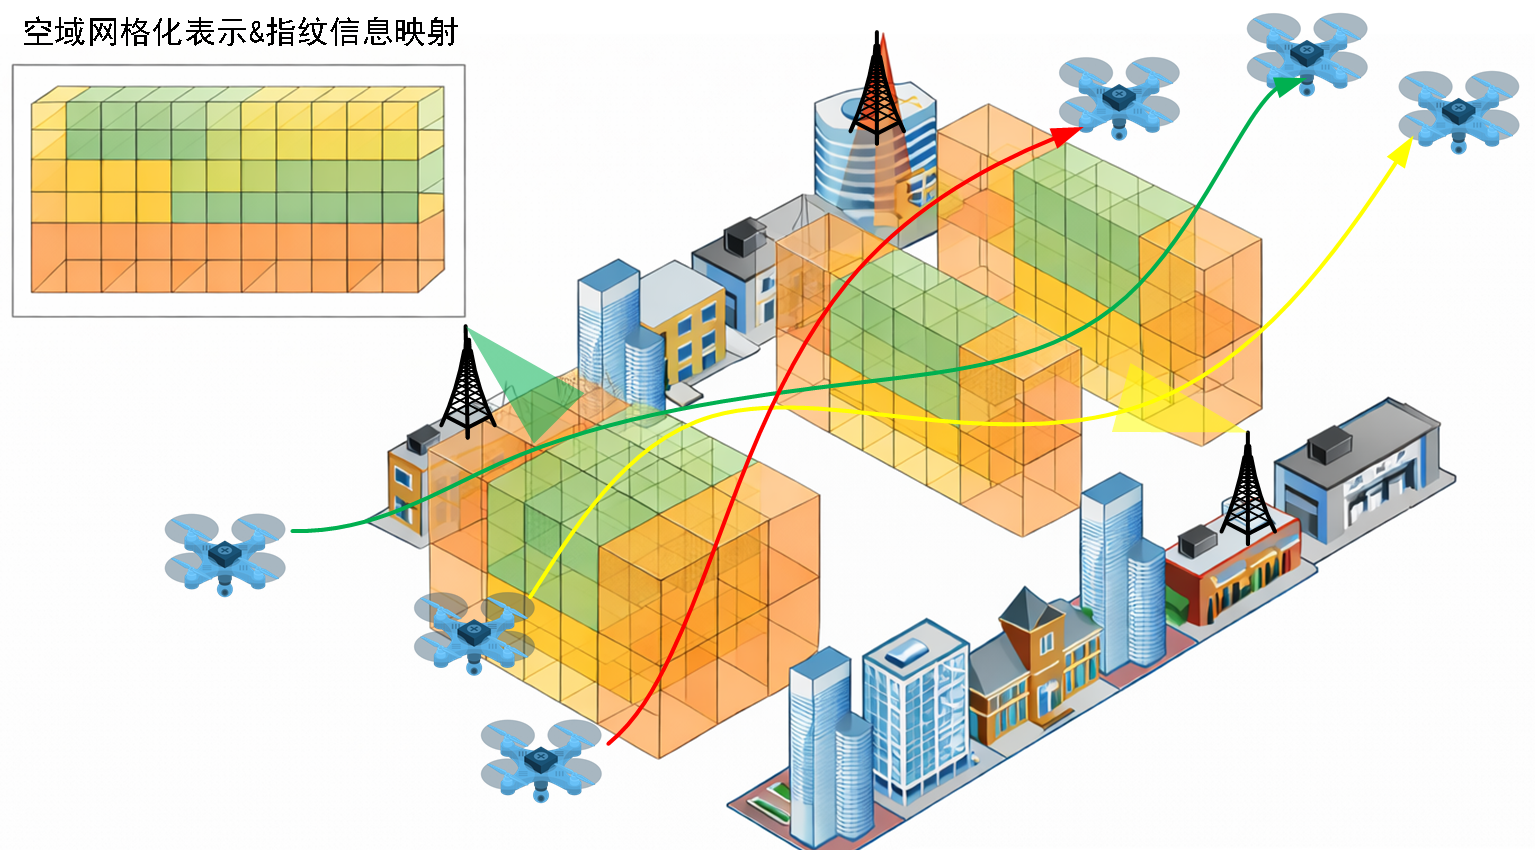
\includegraphics[width=\columnwidth]{figures/urban_clf_framework.png}
\caption{Urban CLF-aided multi-UAV trajectory planning framework.}
\label{fig:urban_clf_framework}
\end{figure}

\subsection{Communication--Localization Fingerprint}

To jointly characterize spatial communication and localization performance in urban environments, we define the communication--localization fingerprint (CLF) of each feasible voxel $v_i\in\mathbf{V}_{\mathrm{feas}}$ as
\begin{equation}
F(v_i)=\{f_{\mathrm{comm}}(v_i),f_{\mathrm{loc}}(v_i)\},\quad v_i\in\mathbf{V}_{\mathrm{feas}},
\end{equation}
where $f_{\mathrm{comm}}(v_i)$ and $f_{\mathrm{loc}}(v_i)$ are the communication and localization fingerprints, respectively.

A line-of-sight (LoS) link exists between $v_i$ and BS $m_k$ if the connecting segment is occlusion-free and within the maximum communication range. Let $\mathbf{M}_i$ denote the set of LoS-accessible BSs for voxel $v_i$.

For communication, the service quality is measured by the maximum achievable capacity among $\mathbf{M}_i$. For the link between $v_i$ and $m_k$, the signal-to-noise ratio is
\begin{equation}
\mathrm{SNR}_{i,k}=\frac{P_kG_{i,k}}{\sigma_0^2},
\end{equation}
where $\sigma_0^2$ is the noise power, $G_{i,k}=\beta_0\,d(\mathbf{c}_i^v,\mathbf{p}_k^m)^{-\alpha}$ is the channel gain, $\beta_0$ is the reference-distance gain, and $\alpha$ is the path-loss exponent. The achievable capacity is $R_{i,k}=B\log_2(1+\mathrm{SNR}_{i,k})$, where $B$ is the system bandwidth. The communication performance of $v_i$ is then
\begin{equation}
C(v_i)=\max_{m_k\in\mathbf{M}_i}R_{i,k}.
\end{equation}

For localization, time difference of arrival (TDOA) is adopted. Based on the Cram\'er--Rao lower bound (CRLB) of TDOA localization~\cite{ref16}, the localization error metric is $L(v_i)=\sqrt{\mathrm{CRLB}(v_i)}$.

To unify the two metrics, we construct normalized fingerprints via the sigmoid mapping. Let $S(x)=1/(1+e^{-x})$ and define
\begin{equation}
\Phi(x;\tau,\alpha)=\frac{S(\alpha(x-\tau))-S(-\alpha\tau)}{1-S(-\alpha\tau)}.
\end{equation}
The communication and localization fingerprints are then
\begin{equation}
f_{\mathrm{comm}}(v_i)=
\begin{cases}
\Phi(C(v_i);C_{\mathrm{th}}-\delta_C,\alpha_C), & |\mathbf{M}_i|\ge 1,\\
0, & \mathrm{otherwise},
\end{cases}
\end{equation}
\begin{equation}
f_{\mathrm{loc}}(v_i)=
\begin{cases}
\Phi(1/L(v_i);1/(L_{\mathrm{th}}+\delta_L),\alpha_L), & |\mathbf{M}_i|\ge 4,\\
0, & \mathrm{otherwise},
\end{cases}
\end{equation}
where $C_{\mathrm{th}}$, $L_{\mathrm{th}}$ are the communication and localization performance thresholds, and $\delta_C,\alpha_C,\delta_L,\alpha_L$ are the corresponding offset and slope parameters. When $|\mathbf{M}_i|<4$, the voxel lacks sufficient BSs for 3-D TDOA localization, so $f_{\mathrm{loc}}(v_i)=0$.

\subsection{UAV Mobility Model}

In the discretized airspace, each UAV can only select its next voxel from the adjacent feasible voxel set $\mathbf{V}_n^{\mathrm{adj}}(t)$ of its current voxel $v_n(t)$ at each time slot. Consequently, a UAV trajectory is a sequence of discrete voxel centers. To respect flight speed constraints, the action set is restricted to the 26-neighborhood and hovering. For a cubic voxel with edge length $\Delta r$, the single-step displacement takes values in $\{0,\Delta r,\sqrt{2}\Delta r,\sqrt{3}\Delta r\}$, corresponding to face-adjacent, edge-adjacent, corner-adjacent moves, and hovering, respectively. The equivalent flight speed $V_n(t)$ is thus quantized to the finite set $\{0,\Delta r/\Delta t,\sqrt{2}\Delta r/\Delta t,\sqrt{3}\Delta r/\Delta t\}$.

For energy consumption, the UAV is approximated as moving at constant speed along the straight line connecting adjacent voxel centers within each time slot. The propulsion power $P(V_n(t))$ follows the rotary-wing UAV power model in~\cite{ref17}. The single-step flight energy is $E_n^{\mathrm{fly}}(t)=P(V_n(t))\cdot\Delta t$, and the total flight energy of UAV $u_n$ over the planning horizon is $E_n^{\mathrm{fly}}=\sum_{t=1}^{T}E_n^{\mathrm{fly}}(t)$, where $T$ is the total number of time slots within the planning horizon. Since $V_n(t)$ only takes a finite set of discrete values, the single-step energy of each action can be precomputed offline and used in the subsequent reward function design.

\subsection{Multi-UAV Planning Problem}

The multi-UAV cooperative trajectory planning problem aims to select, for each UAV at each time slot, a feasible next voxel such that the multi-UAV system achieves favorable communication performance, localization performance, and energy efficiency during trajectory execution while satisfying all constraints. The optimization problem is formulated as
\begin{equation}
\begin{aligned}
\max_{\{v_n(t)\}}\quad &
\sum_{n=1}^{|\mathbf{U}|}\Big\{\sum_{t=1}^{T}\big(w_Cf_{\mathrm{comm}}(v_n(t))
+w_Lf_{\mathrm{loc}}(v_n(t))\big)-w_EE_n^{\mathrm{fly}}\Big\}\\
\mathrm{s.t.}\quad & v_n(t)\in\mathbf{V}_{\mathrm{feas}}\cap\mathbf{V}_n^{\mathrm{adj}}(t-1),\ \forall\,n,t;\\
& v_n(t)\neq v_{n'}(t),\ \forall\,n\neq n';\\
& v_n(0)=v_n^{\mathrm{start}},\ v_n(T)=v_n^{\mathrm{end}}.
\end{aligned}
\end{equation}
Here, $w_E$, $w_C$, and $w_L$ are the energy penalty, communication demand, and localization demand factors, respectively, with $w_C+w_L=1$. The constraints respectively confine each UAV to a feasible voxel adjacent to its previous one, forbid two UAVs from sharing a voxel (flight safety), and fix the start and target voxels within the finite horizon $T$.

Although the CLF map is constructed offline, each UAV can only access local information during the execution phase. The problem is therefore a partially observable multi-agent sequential decision-making problem. In the next section, we further model it as a decentralized partially observable Markov decision process (Dec-POMDP) and solve it using a CTDE-based MARL framework.

\section{Proposed Algorithm}

Under the CTDE framework, MARL algorithms are employed to solve the optimization problem formulated in Section~II. This letter adopts multi-agent proximal policy optimization (MAPPO) as the concrete instantiation of the Dec-POMDP. The overall CTDE-based MARL architecture is illustrated in Fig.~\ref{fig:ctde_marl_framework}.

\begin{figure}[t]
\centering
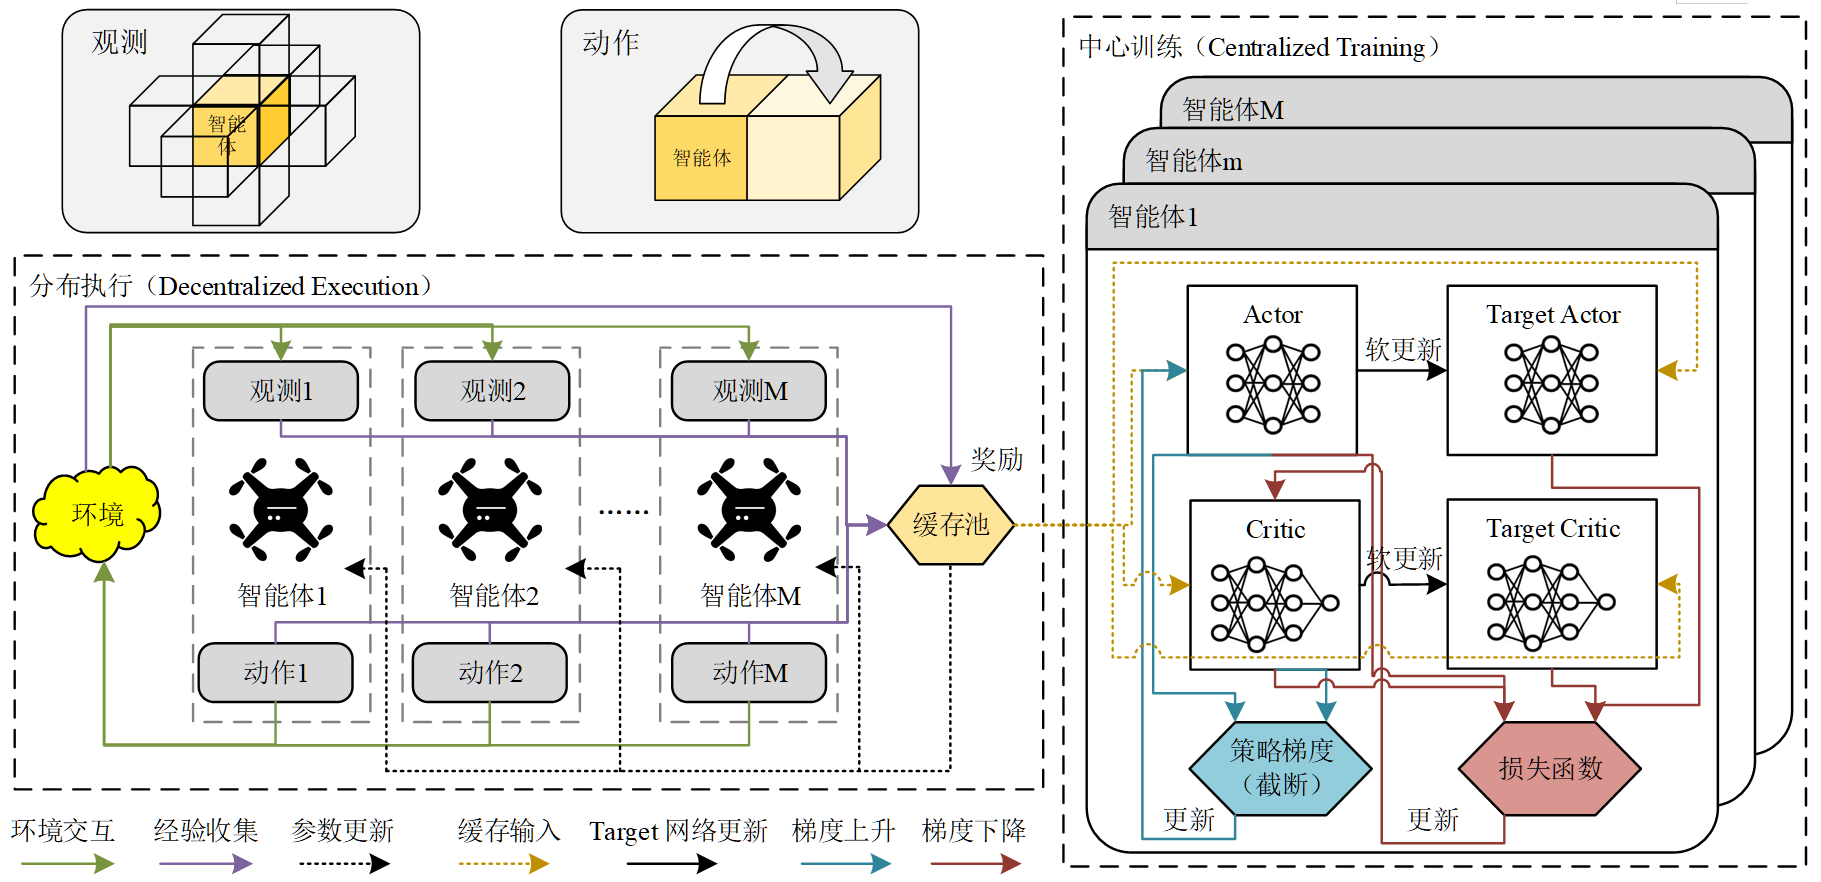
\includegraphics[width=\columnwidth]{figures/ctde_marl_framework.png}
\caption{CTDE-based MARL framework for CLF-aided multi-UAV trajectory planning.}
\label{fig:ctde_marl_framework}
\end{figure}

The design is detailed as follows.

\noindent\textbf{1. State space.}
At time slot $t$, the global state of the system consists of all UAVs' voxel positions and their corresponding CLF values, defined as
\begin{equation}
s(t)=\{v_n(t),F(v_n(t))\}_{n=1,\cdots,|\mathbf{U}|}.
\end{equation}
During decentralized execution, the local observation of UAV $u_n$ is defined as
\begin{equation}
o_n(t)=\{v_n(t),F(v_n(t)),\mathbf{V}_n^{\mathrm{adj}}(t),F(\mathbf{V}_n^{\mathrm{adj}}(t))\},
\end{equation}
where $\mathbf{V}_n^{\mathrm{adj}}(t)$ and $F(\mathbf{V}_n^{\mathrm{adj}}(t))$ are respectively the set of adjacent voxels of $v_n(t)$ and their fingerprint information.

\noindent\textbf{2. Action space.}
Each UAV moves in the discrete grid space, and its action is defined as
\begin{equation}
a_n(t)\in\mathcal{A}_n=\{\mathbf{V}_n^{\mathrm{adj}}(t)\}.
\end{equation}
The action essentially selects the next voxel position from the feasible adjacent voxel set of the current voxel, i.e., $v_n(t)\xrightarrow{a_n(t)}v_n(t+1)$.

\noindent\textbf{3. Reward design.}
This letter constructs a team-averaged immediate reward function based on voxel fingerprint information. To ensure that all components are comparable under a common scale, the communication and localization fingerprints are directly used in their normalized forms, and the energy term is individually normalized. The immediate reward function is defined as
\begin{equation}
\begin{aligned}
r(t)=&\frac{1}{|\mathbf{U}|}\sum_{n}\Big\{X_n(t)\Big[
 w_C(f_{\mathrm{comm}}(v_n(t))-1)\\
&+w_L(f_{\mathrm{loc}}(v_n(t))-1)-w_E\widetilde{E}_n(t)-\delta_n^{\mathrm{coll}}(t)\Big]\\
&+r_{\mathrm{arr}}\big[X_n(t-1)-X_n(t)\big]\Big\}.
\end{aligned}
\end{equation}
The first two lines form the per-step service--energy--safety cost, gated by the arrival indicator $X_n(t)$ so that a UAV stops accruing cost once it reaches its target. The last term is a one-off arrival bonus $r_{\mathrm{arr}}>0$ granted at the single time slot when $X_n$ transitions from $1$ to $0$ (i.e., the step on which UAV $u_n$ first reaches $v_n^{\mathrm{end}}$), which makes goal completion the optimal terminal behavior under the otherwise non-positive per-step reward.
Here, $X_n(t)$ is an arrival-status indicator variable defined as
\begin{equation}
X_n(t)=
\begin{cases}
1, & v_n(t)\neq v_n^{\mathrm{end}};\\
0, & \mathrm{otherwise},
\end{cases}
\end{equation}
which indicates whether UAV $u_n$ remains in an uncompleted mission state. When $X_n(t)=0$, the UAV is considered to have reached its target voxel; its action is locked to hovering and it no longer accumulates communication fingerprint, localization fingerprint, or flight energy cost.

$\widetilde{E}_n(t)$ is the normalized energy penalty defined as
\begin{equation}
\widetilde{E}_n(t)=\frac{E_n(t)}{E_{\max}},
\end{equation}
where $E_n(t)$ is the single-step flight energy and $E_{\max}$ is the maximum single-step energy (corresponding to corner-adjacent movement).

$\delta_n^{\mathrm{coll}}(t)$ is the penalty for multiple UAVs occupying the same voxel, defined as
\begin{equation}
\delta_n^{\mathrm{coll}}(t)=\lambda_{\mathrm{coll}}I_{\mathrm{coll}}(v_n(t)),
\end{equation}
where $\lambda_{\mathrm{coll}}$ is the collision penalty intensity and $I_{\mathrm{coll}}(v_n(t))$ is the collision indicator function defined as
\begin{equation}
I_{\mathrm{coll}}(v_n(t))=
\begin{cases}
1, &\begin{aligned}[t]
&\exists n'\neq n,\ \text{s.t. }v_n(t)=v_{n'}(t)\ \text{or}\\
&v_n(t)=v_{n'}(t-1)\ \text{and}\ v_n(t-1)=v_{n'}(t);
\end{aligned}\\
0, & \mathrm{otherwise}.
\end{cases}
\end{equation}
The collision indicator captures two types of conflicts: co-voxel occupancy and edge-swap crossing between adjacent time slots.

In summary, the reward function exploits the normalized nature of voxel fingerprints to achieve a unified metric for communication and localization performance, and constrains flight energy and flight safety under a common scale through the normalized energy term and the per-UAV collision term.

Based on the above state space, action space, and reward function designs, the MAPPO algorithm proceeds as follows.

\begin{algorithm}[!t]
\caption{CLF-Aided Multi-UAV Trajectory Planning via MAPPO}
\label{alg:clf_mappo}
\scriptsize
\begin{algorithmic}
\REQUIRE CLF map $F(v_i)$, feasible voxel set $\mathbf{V}_{\mathrm{feas}}$,
start/goal voxels $v_n^{\mathrm{start}}$, $v_n^{\mathrm{end}}$,
and MAPPO hyperparameters.

\ENSURE Shared policy network $\pi_{\theta}$.

\STATE Initialize shared actor $\theta$ and centralized critic $\phi$.

\REPEAT
    \STATE Reset UAV positions $v_n(0)\leftarrow v_n^{\mathrm{start}}$ and clear buffer $\mathcal{D}$.

    \FOR{$t=0,\ldots,T-1$}
        \STATE Each UAV constructs $o_n(t)$ from local CLF observations and selects a feasible action
        $a_n(t)\sim\pi_{\theta}(\cdot\mid o_n(t))$.
        \STATE Execute joint action, obtain team reward $r(t)$, observe $s(t+1)$, and store transition in $\mathcal{D}$.
        \IF{all UAVs reach their target voxels}
            \STATE \textbf{break}
        \ENDIF
    \ENDFOR

    \STATE Compute GAE advantages $\hat{A}(t)$ and returns $\hat{R}(t)$.
    \STATE Update actor $\theta$ using PPO clipped objective and update critic $\phi$ using value loss.

\UNTIL{episode $=Epi_{\max}$}
\end{algorithmic}
\end{algorithm}

\section{Experimental Evaluation}

Simulations are conducted in a $600\,\mathrm{m}\times600\,\mathrm{m}\times150\,\mathrm{m}$ urban low-altitude scenario with 15 buildings and 12 ground BSs. The 3-D airspace is voxelized, and UAVs are restricted to feasible voxels satisfying obstacle avoidance, altitude bounds ($h_{\min}=60\,\mathrm{m}$, $h_{\max}=120\,\mathrm{m}$), and a safety margin $d_{\min}^{\mathrm{safety}}=5\,\mathrm{m}$. The communication and localization thresholds $C_{\mathrm{th}}$ and $L_{\mathrm{th}}$ are calibrated automatically from the medians of $C(v_i)$ and $1/L(v_i)$ over all feasible voxels, so that the sigmoid transition zones each span roughly $30\%$--$70\%$ of the feasible space. MAPPO hyperparameters are: discount $\gamma=0.99$, GAE $\lambda=0.95$, PPO clip $\epsilon=0.2$, actor and critic learning rates $3\times10^{-3}$ and $5\times10^{-3}$, and hidden width 128. Each agent is trained for 4000 episodes; the navigation horizon and shaping coefficients are scaled with $1/\Delta r$ to maintain a consistent physical travel budget across resolutions.

\begin{figure}[t]
\centering
\includegraphics[width=\columnwidth]{outputs/policy_comparison.png}
\caption{3-D trajectories (left) and per-step CLF quality (right) of three planners. Line styles distinguish planning strategies; colors identify individual UAVs.}
\label{fig:policy}
\end{figure}

Fig.~\ref{fig:policy} compares the proposed CLF-aware MAPPO against two baselines: a CLF-blind geodesic shortest-path reference and a MAPPO ablation trained without CLF reward. All three planners achieve full arrival, ruling out reachability as a confounding factor. The geodesic reference crosses the city directly, ignoring communication and localization quality. The no-CLF MAPPO learns efficient navigation but remains blind to service fingerprints. In contrast, the proposed CLF-aware MAPPO actively detours around fingerprint-degraded regions, achieving markedly higher mean $f_{\mathrm{comm}}$ and $f_{\mathrm{loc}}$ at only a modest path-length cost.

\begin{figure}[t]
\centering
\includegraphics[width=0.88\columnwidth]{outputs/algo_return_only.png}
\caption{Team episode return versus training episodes for MAPPO, MAA2C, and IPPO on the CLF task. Shading denotes $\pm 1$ std.\ over all 8 seeds.}
\label{fig:algo}
\end{figure}

Fig.~\ref{fig:algo} isolates the algorithmic factors behind planning performance. MAPPO attains the highest team episode return with the smallest inter-seed variance, indicating both the best and the most reliable convergence. IPPO, which replaces the centralized critic with per-agent critics, performs substantially worse, confirming that global state aggregation during training is essential in this partially observable multi-agent setting. MAA2C retains the centralized critic but drops PPO clipping; it reaches a competitive average return yet with markedly larger seed-to-seed variance, indicating that the trust-region clip mainly stabilizes training rather than setting the performance ceiling. Across arrived UAVs, MAPPO achieves balanced fingerprint quality of $f_{\mathrm{comm}}=0.46$ and $f_{\mathrm{loc}}=0.30$.

\begin{figure}[t]
\centering
\includegraphics[width=0.88\columnwidth]{outputs/resolution_return_only.png}
\caption{Team episode return versus training episodes for MAPPO under three voxel resolutions ($\Delta r=20/15/10\,\mathrm{m}$; horizon and shaping scaled $\propto 1/\Delta r$). All resolutions share the same episode budget; shading denotes $\pm 1$ std.\ over seeds.}
\label{fig:resolution}
\end{figure}

Fig.~\ref{fig:resolution} examines the effect of voxel resolution on learning dynamics under an equal episode budget. The coarse grid ($\Delta r=20\,\mathrm{m}$) converges fastest and attains the highest team return, as its compact state--action space is readily optimized within the budget. Refining the grid sharply enlarges the state--action space: the finer grids ($\Delta r=15/10\,\mathrm{m}$) climb more slowly and, under the same budget, plateau at a lower return---the $\Delta r=10\,\mathrm{m}$ run is still tracking upward at the budget horizon. This exposes a representation--complexity tradeoff: finer voxelization raises the theoretically attainable service quality but demands substantially more samples to realize, a practical consideration when deploying CLF-based planning at scale.

\begin{figure}[t]
\centering
\includegraphics[width=0.88\columnwidth]{outputs/pareto_clf.png}
\caption{Communication--localization tradeoff frontier obtained by sweeping $w_L$ under $w_C+w_L=1$. Marker color encodes $w_L$; the line traces the monotone frontier.}
\label{fig:pareto}
\end{figure}

Fig.~\ref{fig:pareto} characterizes the inherent tension between communication and localization in urban blockage environments. Five localization weights $w_L\in\{0,0.25,0.5,0.75,1.0\}$ are evaluated, with a fresh MAPPO trained per point. The frontier is monotone: increasing $w_L$ from 0 to 1 raises $f_{\mathrm{loc}}$ from 0.37 to 0.64 while $f_{\mathrm{comm}}$ declines from 0.69 to 0.54. All UAVs reach their targets at every operating point. These results confirm a quantifiable service tradeoff and demonstrate that the CLF framework supports tunable service provisioning without sacrificing task completion.

\section{Conclusion}

This letter proposed a communication--localization fingerprint (CLF)-aided multi-UAV cooperative trajectory planning framework for urban low-altitude environments. By combining an offline CLF map with CTDE-based multi-agent reinforcement learning, cooperative planning under communication, localization, energy, and collision constraints was achieved. To our knowledge, this is the first work to jointly encode communication and localization performance into spatial fingerprints for multi-UAV planning, eliminating repeated online evaluation. Simulation results confirm that the proposed method improves service continuity and trajectory reliability.

\begin{thebibliography}{17}
\footnotesize
\setlength{\itemsep}{0pt}
\setlength{\parskip}{0pt}
\setlength{\parsep}{0pt}

\bibitem{ref1}
F. Liu, Y. Cui, C. Masouros, J. Xu, T. X. Han, Y. C. Eldar, and S. Buzzi, ``Integrated sensing and communications: Toward dual-functional wireless networks for 6G and beyond,'' \emph{IEEE J. Sel. Areas Commun.}, vol. 40, no. 6, pp. 1728--1767, Jun. 2022.

\bibitem{ref2}
Z. Wei, M. Zhu, N. Zhang, L. Wang, Y. Zou, Z. Meng, H. Wu, and Z. Feng, ``UAV-assisted data collection for Internet of Things: A survey,'' \emph{IEEE Internet Things J.}, vol. 9, no. 17, pp. 15460--15483, Sep. 2022.

\bibitem{ref3}
L. Gupta, R. Jain, and G. Vaszkun, ``Survey of important issues in UAV communication networks,'' \emph{IEEE Commun. Surveys Tuts.}, vol. 18, no. 2, pp. 1123--1152, Second Quart. 2016.

\bibitem{ref4}
S. Hayat, E. Yanmaz, and R. Muzaffar, ``Survey on unmanned aerial vehicle networks for civil applications: A communications viewpoint,'' \emph{IEEE Commun. Surveys Tuts.}, vol. 18, no. 4, pp. 2624--2661, Fourth Quart. 2016.

\bibitem{ref5}
Z. Xiao, L. Zhu, Y. Liu, P. Yi, R. Zhang, X.-G. Xia, and R. Schober, ``A survey on millimeter-wave beamforming enabled UAV communications and networking,'' \emph{IEEE Commun. Surveys Tuts.}, vol. 24, no. 1, pp. 557--610, First Quart. 2022.

\bibitem{ref6}
Y. Zeng, R. Zhang, and T. J. Lim, ``Wireless communications with unmanned aerial vehicles: Opportunities and challenges,'' \emph{IEEE Commun. Mag.}, vol. 54, no. 5, pp. 36--42, May 2016.

\bibitem{ref7}
J. Chen, U. Mitra, and D. Gesbert, ``3D urban UAV relay placement: Linear complexity algorithm and analysis,'' \emph{IEEE Trans. Wireless Commun.}, vol. 20, no. 8, pp. 5243--5257, Aug. 2021.

\bibitem{ref8}
X. Yu, Y. Zheng, M. Sheng, Y. Shi, and J. Li, ``Optimizing UAV deployment and access control for integrated localization and communication,'' in \emph{Proc. IEEE Int. Conf. Commun. (ICC)}, 2025, pp. 6615--6620.

\bibitem{ref9}
Z. Wang, J. Zhao, F. He, W. Jia, W. Jin, and Q. Wu, ``A hierarchical MADRL framework for joint resource allocation and trajectory design in UAV enabled multi-static ISAC networks,'' \emph{IEEE Wireless Commun. Lett.}, vol. 15, pp. 1325--1329, Jan. 2026.

\bibitem{ref10}
X. Xu, H. Xu, D. Wei, W. Saad, M. Bennis, and M. Chen, ``Transformer-based collaborative reinforcement learning for fluid antenna system (FAS)-enabled 3D UAV positioning,'' \emph{IEEE J. Sel. Areas Commun.}, vol. 44, pp. 1128--1143, 2026.

\bibitem{ref11}
Y. Xie, L. Wang, Z. Chang, L. Xu, S. Bi, and Z. Han, ``GeoAgg-HSAC: An RL-based framework for trajectory and resource optimization in mountainous UAV integrated localization and communication networks,'' \emph{IEEE Trans. Wireless Commun.}, vol. 25, pp. 6507--6520, 2026.

\bibitem{ref12}
Q. Gao, R. Zhong, H. Shin, and Y. Liu, ``MARL-based UAV trajectory and beamforming optimization for ISAC system,'' \emph{IEEE Internet Things J.}, vol. 11, no. 24, pp. 40492--40504, Dec. 2024.

\bibitem{ref13}
D. Gesbert, O. Esrafilian, J. Chen, R. Gangula, and U. Mitra, ``UAV-aided RF mapping for sensing and connectivity in wireless networks,'' \emph{IEEE Wireless Commun.}, pp. 116--122, Aug. 2023.

\bibitem{ref14}
O. Esrafilian, R. Gangula, and D. Gesbert, ``UAV-aided wireless node localization using hybrid radio channel models,'' in \emph{Proc. IEEE Int. Conf. Commun. Workshops (ICC Workshops)}, 2022, pp. 1083--1088.

\bibitem{ref15}
P. Yi, L. Zhu, L. Zhu, Z. Xiao, Z. Han, and X.-G. Xia, ``Joint 3-D positioning and power allocation for UAV relay aided by geographic information,'' \emph{IEEE Trans. Wireless Commun.}, vol. 21, no. 10, pp. 8148--8162, Oct. 2022.

\bibitem{ref16}
J. A. del Peral-Rosado, J. A. Lopez-Salcedo, G. Seco-Granados, F. Zanier, and M. Crisci, ``Achievable localization accuracy of the positioning reference signal of 3GPP LTE,'' in \emph{Proc. Int. Conf. Localization GNSS (ICL-GNSS)}, 2012, pp. 1--6.

\bibitem{ref17}
Y. Zeng, J. Xu, and R. Zhang, ``Energy minimization for wireless communication with rotary-wing UAV,'' \emph{IEEE Trans. Wireless Commun.}, vol. 18, no. 4, pp. 2329--2345, Apr. 2019.

\end{thebibliography}

\end{document}
